\subsection{Size, power and familywise error: simulations}\label{sec:testing-sim}

This subsection checks the tests of Section~\ref{sec:testing} by simulation. We ask whether the Wald tests have their nominal size, whether the simultaneous procedures control the familywise error rate (FWER) over the $K=108$ contrasts, whether the label budgets predicted by the power formula are the ones observed, and whether allocating labels for power helps. Full tables are in Supplementary Section~\SIref{si:testing-sim}.

\paragraph{Set-up.} The synthetic population is the generative model of the non-smooth simulation (five Gaussian covariates, a group with prevalence $0.3$, a logistic label model) with nine fixed scoring rules, so there are $36$ pairs and $108$ contrasts. To have contrasts that are exactly zero in the population without making them trivial, four rules use the covariate $x_4$, which does not enter the label model, and each has a twin that uses $x_5$ instead, with the same weights, scale and group offset. Because $x_4$ and $x_5$ are exchangeable and independent of $(Y,G)$, a rule and its twin have the same TPR gap, FPR gap and error rate, so the three contrasts of each of the four pairs are zero: $12$ true nulls, whereas the twins' predictions differ on a large part of every pool. The population values come from $2\times10^{7}$ draws. We compare SRS and PATTERN with the plug-in estimator and PATTERN-DIF, with the variance estimators of Section~\ref{sec:design}. Pools of $N\in\{2000,8000\}$ units are drawn anew in every replication, with $L\in\{250,500,1000,2000\}$ and $L\le N/4$ (six cells), and $R=1000$ replications per cell. The pool-conditional test targets the contrast of the pool, the two-phase test the population contrast with the variance of Section~\ref{sec:population}. On the eleven cached real pools the truth is the pool contrast computed from all labels. Simultaneous procedures use $\alpha=0.05$; the max-$t$ critical value is the $0.95$ quantile of $\max_k|X_k|$ for $X\sim N(0,\hat R)$, from $20{,}000$ draws with a fixed seed. With $R=1000$ the Monte Carlo standard error of a rejection rate near $0.05$ is $0.007$, and the largest of $108$ such rates from a perfectly calibrated test has mean $0.068$ (at $\alpha=0.01$ and $0.10$: $0.019$ and $0.125$), so we compare ``max'' columns with these values and not with the nominal level.

\paragraph{Size.} Table~\ref{tab:test-size} and Figure~\ref{fig:testing-sim}(a) give the results for PATTERN-DIF. The two-sided Wald test of the true value has mean rejection rate $0.048$ to $0.053$ at $\alpha=0.05$ in all six cells, for the pool-conditional test of the pool contrast and for the two-phase test of the population contrast ($0.009$ to $0.012$ and $0.096$ to $0.104$ at $\alpha=0.01$ and $0.10$). The worst contrast is rejected in $0.063$ to $0.074$ of the replications; the largest value, $0.074$, is just above the $0.068$ expected from noise alone, and we do not read it as a failure. The plug-in estimators with SRS and PATTERN behave in the same way (mean $0.048$ to $0.056$), SRS being slightly liberal at $L=250$ (worst contrast $0.08$). One-sided tests at the boundary of the null reject in $0.048$ to $0.055$ of the replications on average (all three designs) (non-inferiority at the boundary is the one-sided test with margin equal to the true value), and the TOST at the boundary of the equivalence region is conservative on average ($0.02$ to $0.05$ at $\alpha=0.05$), as it should be when the margin is small relative to the standard error (Supplementary Table~\SIref{tab:test-onesided-full}). The pool term matters for the target, not for the test of the target actually chosen. The pool-conditional test of the \emph{population} value rejects in $0.060$ to $0.175$ of the replications at nominal $0.05$, increasing with $\varpi=\hat V_{\rm pool}/\hat V_{\rm design}$ (from $0.08$ to $1.19$), while the two-phase test stays at $0.05$ (Supplementary Table~\SIref{tab:test-size-popdesign}).

\begin{table}[t]
\centering\footnotesize
\caption{PATTERN-DIF, synthetic population, $R=1000$ pools per row. Size: rejection rate of the two-sided Wald test of the true value at nominal $0.05$ (pool-conditional test of the pool contrast; two-phase test of the population contrast), mean and maximum over the $108$ contrasts (the maximum of a calibrated test has mean $0.068$). $\varpi$: median estimated $V_{\rm pool}/V_{\rm design}$. FWER: probability of rejecting at least one of the $12$ true nulls of $H_k:\theta_k=0$, $k=1,\dots,108$, at familywise level $0.05$ (population target).}\label{tab:test-size}
\resizebox{\textwidth}{!}{\begin{tabular}{rr r rr rr rrrr}\toprule
 & & & \multicolumn{2}{c}{Size, pool value} & \multicolumn{2}{c}{Size, population value} & \multicolumn{4}{c}{FWER, population nulls} \\
$N$ & $L$ & $\varpi$ & mean & max & mean & max & Unadj. & Bonf. & Holm & Max-$t$ \\\midrule
2{,}000 & 250 & 0.39 & 0.051 & 0.066 & 0.051 & 0.067 & 0.398 & 0.006 & 0.008 & 0.009 \\
 & 500 & 1.11 & 0.053 & 0.069 & 0.051 & 0.069 & 0.406 & 0.007 & 0.008 & 0.008 \\
\addlinespace
8{,}000 & 250 & 0.08 & 0.052 & 0.069 & 0.051 & 0.066 & 0.353 & 0.005 & 0.006 & 0.009 \\
 & 500 & 0.20 & 0.048 & 0.064 & 0.049 & 0.067 & 0.375 & 0.002 & 0.003 & 0.004 \\
 & 1000 & 0.46 & 0.050 & 0.069 & 0.048 & 0.063 & 0.386 & 0.007 & 0.011 & 0.009 \\
 & 2000 & 1.19 & 0.052 & 0.074 & 0.053 & 0.071 & 0.450 & 0.006 & 0.008 & 0.008 \\
\bottomrule\end{tabular}
}
\end{table}

\paragraph{Familywise error and power.} With only $12$ true nulls among $108$ hypotheses the familywise error of every adjusted procedure is far below $0.05$ (Table~\ref{tab:test-size}, FWER columns: $0.002$ to $0.011$ for Bonferroni, Holm and max-$t$, against $0.35$ to $0.45$ unadjusted), because the correction is for $108$ tests whereas the null set is small. That is conservative but not informative about tightness, so we also test the family in which every hypothesis is true ($H_k:\theta_k=\theta_k^{\rm true}$), where the FWER is one minus the simultaneous coverage (Figure~\ref{fig:testing-sim}(b), Supplementary Table~\SIref{tab:test-fwer-full}). For PATTERN-DIF the unadjusted tests reject at least one true hypothesis in $0.76$ to $0.81$ of the replications for the pool target and in $0.82$ to $0.90$ for the population target, so $108$ unadjusted intervals almost never cover simultaneously. Bonferroni and Holm (identical here) have FWER $0.03$ to $0.05$, and max-$t$ $0.05$ to $0.07$ (mean $0.058$ for both targets). Max-$t$ is therefore slightly anticonservative, by about one percentage point, in line with its critical value being only $3\%$ below the Bonferroni value (about $3.4$ against $3.5$): the contrasts are only moderately correlated, so the gain is small, and the estimated correlation matrix adds noise. The anticonservatism is larger for the plug-in estimators with small budgets (SRS: FWER up to $0.09$ at $N=2000$, $L=250$). The cell with the largest value for PATTERN-DIF ($0.07$) is within three Monte Carlo standard errors of $0.05$. The power of the three procedures against the $80$ false nulls with $|\theta_k|\ge0.02$ is higher for Holm and max-$t$ than for Bonferroni in every cell, by $0.01$ to $0.03$, and neither of the two dominates: max-$t$ is ahead at small budgets (PATTERN-DIF, $N=2000$, $L=250$: $0.20$ against $0.19$ for Holm and $0.18$ for Bonferroni) and Holm at large ones ($N=8000$, $L=2000$: $0.68$, $0.67$, $0.66$ for Holm, max-$t$, Bonferroni). Holm is never less powerful than Bonferroni. PATTERN-DIF has the highest power at every budget (Bonferroni power $0.52$ against $0.36$ for SRS at $N=8000$, $L=1000$).

\paragraph{Real pools.} On the eleven cached real pools (35 setting--budget cells, $R=400$, truth from the pool labels; the $K$ contrasts that are not identically zero, so $K=108$, except $57$ in Law school) we measured the simultaneous coverage of the family of pool contrasts. For PATTERN-DIF the unadjusted intervals cover all contrasts at once in only $0.20$ to $0.33$ of the replications on average over cells (by budget), Bonferroni and Holm in $0.93$, $0.96$, $0.97$ and $0.98$ at $L=250$, $500$, $1000$, $2000$, and max-$t$ in $0.90$, $0.93$, $0.94$ and $0.945$. Over all cells the means are $0.954$ (Bonferroni, Holm) and $0.923$ (max-$t$); the Monte Carlo standard error is $0.011$. Max-$t$ is thus not conservative on real pools but falls short of its level, by $0.03$ on average and by more at small budgets, and the shortfall is concentrated in a few cells: it is below $0.90$ in four of the $35$ (Law school at $L=250$ and $500$ with $0.65$ and $0.89$, MAGIC at $L=250$ with $0.885$, Spambase at $L=250$ with $0.897$); Bonferroni is below $0.93$ in three (Law school $L=250$: $0.72$, MAGIC $L=250$ and $500$). These are the cells in which the main study found worst-contrast coverage below nominal, so the failure is that of the individual intervals at small budgets, not of the max-$t$ construction. With the zero-variance floor of Section~\ref{sec:design} the minimum over cells rises from $0.72$ to $0.92$ for Bonferroni and from $0.65$ to $0.89$ for max-$t$ (mean $0.934$). The plug-in estimators are much worse (mean Bonferroni coverage $0.67$ for SRS and $0.91$ for PATTERN), as in the main study. The critical value of max-$t$ is on average $5\%$ below the Bonferroni value for these real contrasts, which are more strongly correlated than the synthetic ones (Supplementary Tables~\SIref{tab:test-real-cover-full} and~\SIref{tab:test-real-cover-summary}).

\paragraph{Power curves and label budgets.} For six contrasts per setting (selected so that the predicted budgets for SRS and PATTERN-DIF both fall in the grid $200\le L\le\min(4000,N/4)$; $R=1000$ labelled samples per budget, pool-conditional target) we estimated the power of the two-sided test of $H_0:\theta_k=0$ at seven budgets and interpolated in $\log L$ to the budget for $80\%$ power. We compare the ratio $L_{\rm SRS}/L_{\rm DIF}$ with the prediction from the power function with the exact finite-pool variances (computed with the pool labels and the allocation actually used). Figure~\ref{fig:testing-sim}(c) and Table~\ref{tab:test-power} show close agreement: over $49$ contrasts in nine settings the median of observed over predicted is $1.00$ (quartiles $0.97$ and $1.02$), all ratios lie within $\pm20\%$ and the rank correlation is $0.99$; absolute budgets agree equally well ($0.99$ and $1.00$ for SRS and PATTERN-DIF). Two contrasts were censored (power never reached $80\%$ on the grid). The asymptotic prediction by the ratio of variances is slightly too high. The ratio of the variances of SRS and PATTERN-DIF at the budget of PATTERN-DIF is $2.9$ to $6.0$ across settings, and the observed budget ratio is about $0.88$ times it (range $0.78$ to $1.08$), because the finite-pool factor $1/L-1/N$ makes the variance of SRS fall faster than $1/L$ at the budgets reached; the sample-size formula that includes it is accurate. The MSE ratio of the main study at $L=500$ is a different quantity and need not agree: it is the efficiency at one budget, and for several settings it exceeds the budget ratio (for example $12.1$ against $4.9$ for Bank marketing), because PATTERN-DIF exhausts small strata as the budget grows.

\begin{table}[t]
\centering\footnotesize
\caption{Label budget for $80\%$ power of the two-sided Wald test of $H_0:\theta_k=0$, ratio of SRS to PATTERN-DIF. $V_{\rm SRS}/V_{\rm DIF}$: ratio of exact variances at the budget of PATTERN-DIF (asymptotic prediction, median over contrasts); predicted: from the power function with the exact variance at each budget; observed: from $R=1000$ simulated power curves; Obs./pred.: median of the per-contrast ratio. Contrasts: number selected per setting.}\label{tab:test-power}
\begin{tabular}{lrrrrr}\toprule
Setting & Contrasts & $V_{\rm SRS}/V_{\rm DIF}$ & Predicted $L_{\rm SRS}/L_{\rm DIF}$ & Observed & Obs./pred.\ \\\midrule
Synthetic pool & 6 & 2.88 & 2.79 & 2.60 & 0.97 \\
Adult (sex) & 6 & 5.97 & 5.40 & 5.35 & 1.02 \\
Adult (race) & 6 & 3.57 & 3.29 & 3.37 & 0.97 \\
Bank marketing & 6 & 5.88 & 4.92 & 4.88 & 1.00 \\
Credit card & 6 & 4.37 & 3.66 & 3.59 & 0.96 \\
MAGIC & 6 & 3.52 & 3.11 & 3.07 & 1.00 \\
EEG eye state & 6 & 4.35 & 3.76 & 3.93 & 1.03 \\
Phoneme & 3 & 2.94 & 2.49 & 2.28 & 0.97 \\
Electricity & 6 & 3.01 & 2.83 & 2.87 & 1.01 \\
\midrule
All & 51 & & 3.29 & 3.35 & 1.00 \\
\bottomrule\end{tabular}

\end{table}

\paragraph{Power-optimal allocation.} For the synthetic pool and three real pools (Adult (sex), Bank marketing, Electricity) with $L\in\{500,1000\}$ we solved the maximin problem of Section~\ref{sec:testing} with the effect sizes as targets, using the true contrasts (an idealisation: in practice they come from a pilot or from planning values). Two target sets were used: E1, the contrasts with $|\theta_k|\ge0.02$ with effect $|\theta_k|$, and E2, all contrasts with a common effect of $0.05$. The solver is certified: the duality gap was below $0.2\%$ in every problem. Compared with the default allocation, the maximin allocation reduces the largest variance-to-effect ratio $\max_kV_k/\delta_k^2$ by a factor of $1.5$ to $2.0$ in the real pools and by $1.05$ on the synthetic pool, where the default is already close to optimal (Supplementary Table~\SIref{tab:test-opt-full}). The power at the worst contrast rises accordingly but from low levels, because the hardest contrasts remain nearly unpowered at these budgets: for E2 it goes from $0.09$ to $0.13$ (Adult (sex), $L=500$), from $0.17$ to $0.23$ (Bank marketing, $L=1000$) and from $0.37$ to $0.65$ (Electricity, $L=1000$), whereas for E1 at $L=1000$ the gains are smaller ($0.12$ to $0.14$ in Adult (sex), none in Bank marketing, $0.15$ to $0.21$ in Electricity). The cost is the mean power and the number of contrasts that reach $80\%$: in Adult (sex) at $L=1000$ the mean power under E2 falls from $0.87$ to $0.79$ and the number of contrasts below $80\%$ rises from $21$ to $35$. Power-optimal design therefore helps the worst-off contrasts and costs the others; it is not a free improvement.

\begin{figure}[t]
\centering
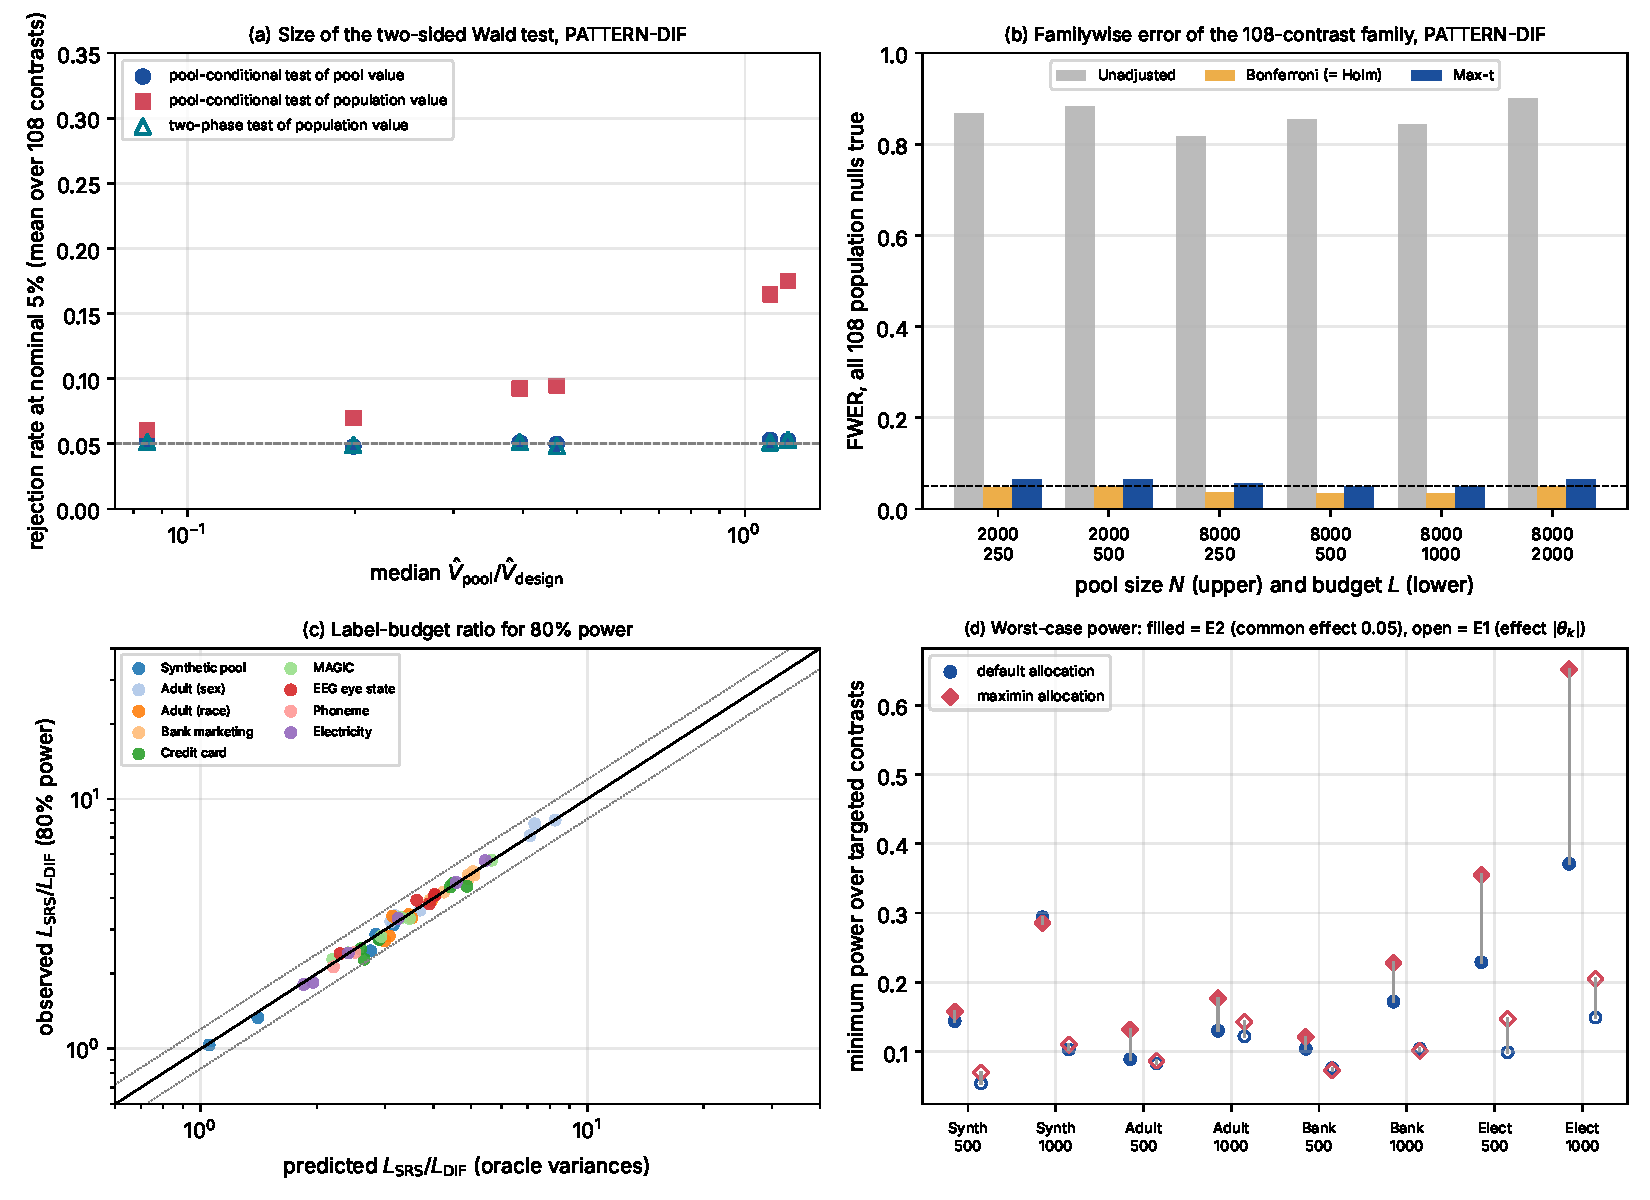
\includegraphics[width=\textwidth]{figures/testing_sim}
\caption{(a) Rejection rate at nominal $5\%$ (mean over $108$ contrasts) against the estimated ratio of pool to design variance. (b) FWER of the family in which all $108$ population hypotheses are true, by cell ($N$ above, $L$ below). (c) Predicted and observed $L_{\rm SRS}/L_{\rm DIF}$ at $80\%$ power, one point per contrast; dotted lines: $\pm20\%$. (d) Minimum simulated power over the targeted contrasts under the default and the maximin allocation (filled: E2, open: E1).}\label{fig:testing-sim}
\end{figure}

\paragraph{Limitations.} The nulls are exact only in the population and there are only $12$ of them, so the adjusted FWER with true nulls is conservative and the all-true family is the demanding check. There is one synthetic design and eleven real pools; the power study uses contrasts whose budgets fall in the grid, and the power-optimal allocation is evaluated with the true effect sizes and the proxy variance model. Max-$t$ uses an estimated correlation matrix of $108$ contrasts and is mildly anticonservative at small budgets. Further limitations are listed in Supplementary Section~\SIref{si:testing-sim}.
